So far, we have looked at linear models of the form
\begin{align}
	Y_i = \beta_0 + \beta_1x_{1i} + \beta_2x_{2i} + \dots + \beta_px_{pi} + \epsilon_i\notag
\end{align}
In this lecture, we extend this concept:
\begin{itemize}
	\item We look at how we can use different types of predictors to capture a wide range of relationships (e.g. capture non-linear relationship with linear model).
	\item We'll think about how to formulate models, depending on their use.
	\item We'll consider some common pitfalls in use of linear models.
\end{itemize}

\begin{example}
	Consider energy usage in houses, based on their size.
	\begin{center}
		\begin{tikzpicture}[scale=0.9]
			\begin{axis}[
				xmin=0, xmax=3, xlabel=$x$,
				ymin=4, ymax=8, ylabel=$y$,
				title=\textbf{Linear fit},
				axis x line=middle,
				axis y line=middle,
				samples=400
			]
			\addplot[blue, mark=x, only marks] coordinates	{
				(0.00,4.00)
				(0.10,4.42)
				(0.20,4.81)
				(0.30,5.18)
				(0.40,5.51)
				(0.50,5.82)
				(0.60,6.11)
				(0.70,6.37)
				(0.80,6.60)
				(0.90,6.81)
				(1.00,7.00)
				(1.10,7.17)
				(1.20,7.31)
				(1.30,7.43)
				(1.40,7.53)
				(1.50,7.61)
				(1.60,7.68)
				(1.70,7.72)
				(1.80,7.75)
				(1.90,7.75)
				(2.00,7.75)
				(2.10,7.72)
				(2.20,7.68)
				(2.30,7.63)
				(2.40,7.56)
				(2.50,7.48)
				(2.60,7.39)
				(2.70,7.28)
				(2.80,7.16)
				(2.90,7.03)
			};
			\addplot[mark=none] {0.96*x+5.4};
			\end{axis}
		\end{tikzpicture}
		\begin{tikzpicture}[scale=0.9]
		\begin{axis}[
		xmin=0, xmax=3, xlabel=$x$,
		ymin=4, ymax=8, ylabel=$y$,
		title=\textbf{Polynomial fit},
		axis x line=middle,
		axis y line=middle,
		samples=400
		]
		\addplot[blue, mark=x, only marks] coordinates	{
			(0.00,4.00)
			(0.10,4.42)
			(0.20,4.81)
			(0.30,5.18)
			(0.40,5.51)
			(0.50,5.82)
			(0.60,6.11)
			(0.70,6.37)
			(0.80,6.60)
			(0.90,6.81)
			(1.00,7.00)
			(1.10,7.17)
			(1.20,7.31)
			(1.30,7.43)
			(1.40,7.53)
			(1.50,7.61)
			(1.60,7.68)
			(1.70,7.72)
			(1.80,7.75)
			(1.90,7.75)
			(2.00,7.75)
			(2.10,7.72)
			(2.20,7.68)
			(2.30,7.63)
			(2.40,7.56)
			(2.50,7.48)
			(2.60,7.39)
			(2.70,7.28)
			(2.80,7.16)
			(2.90,7.03)
		};
		\addplot[mark=none] {0.1089*x^3-1.453*x^2+4.344*x+4};
		\end{axis}
		\end{tikzpicture}
	\end{center}
\end{example}

A simple linear models might tell us that a predictor is important, but it's no good prediction. Model building is a process that includes:
\begin{itemize}
	\item \textbf{Formulating a model:} model structure, we'll look at different types of predictors today.
	\item \textbf{Model fitting:} last two lectures
	\item \textbf{Model evaluation:} Check model assumptions hold, avoid common pitfalls
\end{itemize}

Before formulating a statistical model, it is good practice to explore the data. Look at scatter plots of predictors against the response and predictors against each other. Can help to develop an intuition for model structure. Look at distributions of response and predictors (e.g. look for outliers, can you capture the distribution with your model?) Think about what the model will be used for (e.g. prediction, or simply to find relevant explanatory variables).

\subsection{Types of predictors}

\subsubsection{qualitative vs quantitative}

So far, we have looked at \begriff{quantitative predictors} (numerical variables), e.g. temperature, energy usage, waiting time before computer processes data, ... But we can have \begriff{qualitative predictors} as well (categorical variables), e.g. type of engine, type fuel used, type of processor used, ... These are included in models using \begriff{dummy variables}.

\begin{example}
	Consider the performance $Y_i$ of diesel engines for three different fuel types A, B and C. We use the model $Y_i = \beta_0 + \beta_1x_{1i} + \beta_2x_{2i} + \epsilon_i$, where $x_{1i}$ and $x_{2i}$ are dummy variables such that
	\begin{align}
		x_{1i} &= \begin{cases}
		1 & \text{if fuel B is used} \\ 0 & \text{if not}
		\end{cases} \notag \\
		x_{2i} &= \begin{cases}
		1 & \text{if fuel C is used} \\ 0 & \text{if not}
		\end{cases} \notag 
	\end{align}
	The performance for fuel type A is captured in $\beta_0$.
\end{example}

Qualitative and quantitative predictors can be combined in models.

\begin{example}
	Consider fuel efficiency of car models from the 1950s (\textcolor{blue}{type 1}) and from the 1960s (\textcolor{red}{type 2}), depending on their weight. For car models $i=1,...,n$, we might consider the model $Y_i = \beta_0 + \beta_1x_i + \beta_2w_i + \epsilon_i$, where $Y_i$ is the efficiency in miles per gallon (MPG), $x_i$ is a dummy variable for the car type and $w_i$ is the weight of a car model. We might find:
	\begin{center}
	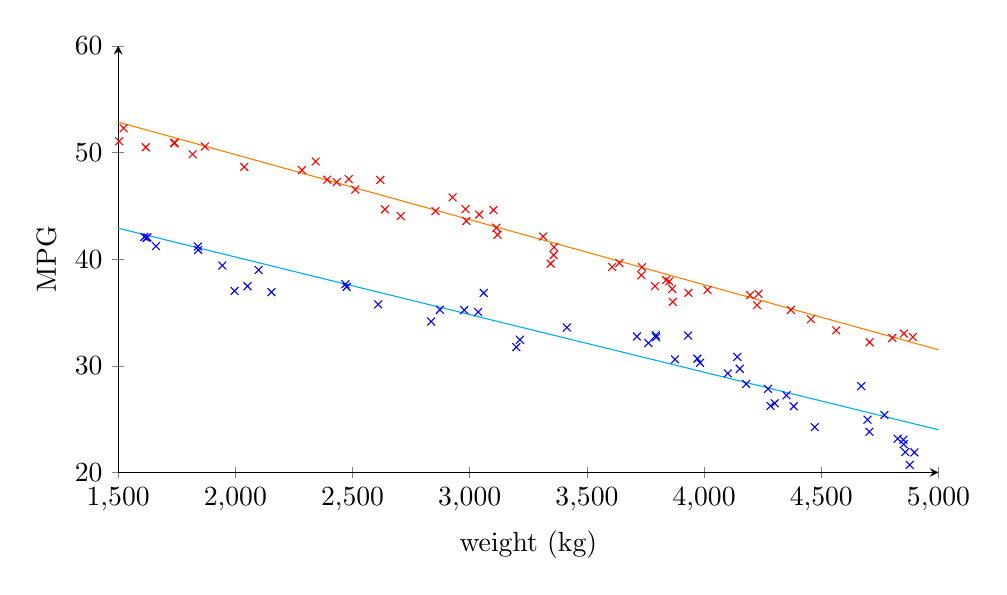
\begin{tikzpicture}
		\begin{axis}[
		xmin=1500, xmax=5000, xlabel=weight (kg),
		ymin=20, ymax=60, ylabel=MPG,
		axis x line=bottom,
		axis y line=left,
		samples = 400,
		height=7cm,
		width=12cm,
		domain=1500:5000
		]
		\addplot[blue, mark=x, only marks] coordinates {
			(1611.41,42.08)
			(1620.56,42.00)
			(1624.99,42.04)
			(1661.60,41.22)
			(1839.96,41.19)
			(1841.39,40.86)
			(1944.45,39.40)
			(1996.60,37.02)
			(2051.65,37.46)
			(2099.15,38.98)
			(2154.05,36.90)
			(2469.23,37.65)
			(2474.74,37.40)
			(2609.85,35.76)
			(2835.45,34.15)
			(2872.79,35.25)
			(2976.16,35.22)
			(3035.61,35.04)
			(3059.55,36.83)
			(3198.81,31.75)
			(3214.18,32.44)
			(3414.09,33.59)
			(3713.26,32.75)
			(3762.10,32.13)
			(3794.17,32.87)
			(3795.09,32.68)
			(3875.57,30.60)
			(3931.90,32.84)
			(3971.16,30.67)
			(3982.78,30.28)
			(4100.96,29.29)
			(4141.40,30.83)
			(4152.09,29.72)
			(4179.31,28.30)
			(4272.73,27.84)
			(4283.20,26.24)
			(4300.98,26.48)
			(4351.53,27.23)
			(4382.10,26.20)
			(4471.95,24.25)
			(4670.27,28.10)
			(4696.82,24.95)
			(4705.07,23.82)
			(4768.98,25.39)
			(4825.78,23.16)
			(4850.08,23.07)
			(4851.27,22.65)
			(4858.22,21.91)
			(4877.11,20.71)
			(4897.07,21.88)
		};
		\addplot[red,mark=x,only marks] coordinates {
			(1504.03,51.05)
			(1523.50,52.27)
			(1617.61,50.49)
			(1737.97,50.88)
			(1740.82,50.90)
			(1817.88,49.83)
			(1869.70,50.56)
			(2037.80,48.64)
			(2284.14,48.35)
			(2342.47,49.15)
			(2391.77,47.45)
			(2432.65,47.22)
			(2483.52,47.50)
			(2511.73,46.52)
			(2618.60,47.43)
			(2638.01,44.67)
			(2705.62,44.04)
			(2853.70,44.50)
			(2926.67,45.79)
			(2982.09,44.69)
			(2985.22,43.58)
			(3040.30,44.18)
			(3100.99,44.60)
			(3113.21,42.94)
			(3118.57,42.29)
			(3313.18,42.12)
			(3345.00,39.58)
			(3358.02,40.38)
			(3359.67,41.13)
			(3607.60,39.26)
			(3638.36,39.63)
			(3731.98,38.49)
			(3734.86,39.25)
			(3790.56,37.47)
			(3837.41,38.04)
			(3851.33,37.91)
			(3863.66,37.21)
			(3866.43,35.99)
			(3932.99,36.84)
			(4014.26,37.12)
			(4195.56,36.63)
			(4225.81,35.69)
			(4231.82,36.74)
			(4369.93,35.24)
			(4455.37,34.36)
			(4563.80,33.32)
			(4705.97,32.20)
			(4802.68,32.61)
			(4851.93,33.02)
			(4890.27,32.70)
		};
		\addplot[cyan,mark=none] {-0.0054*x+51};
		\addplot[orange,mark=none] {-0.0061*x+62};
		\end{axis}
	\end{tikzpicture}
\end{center}
\end{example}

\subsubsection{interaction terms}

\subsubsection{polynomials of predictors}

\subsubsection{data transformations}

\subsection{Pitfalls}